\documentclass{article}
%\usepackage{geometry}
% \geometry{top = 1in, bottom = 1in, left = 1in, right = 1in}
\usepackage[top = 0.7in, bottom = 0.7in, left = 0.7in, right = 0.7in]{geometry}

\usepackage{amsmath,amssymb,amsthm,mathrsfs}

\usepackage{graphicx}

\usepackage{bm}
\usepackage{float}
\usepackage[font=footnotesize,labelfont=bf]{caption}

\usepackage{fancyhdr}
\pagestyle{fancy}
\rhead{\footnotesize {07/26/2012 ; MESA version 4028} }
\chead{\footnotesize {Authors: Jared Brooks, Lars Bildsten, Bill Paxton} }
\lhead{\footnotesize {mesa/star/test\_suite/brown\_dwarf} }

\begin{document}

	\begin{center}
		\begin{Large}
			\textbf{Brown Dwarf}\\
		\end{Large}
	\end{center}
	
        This test is to show that a 0.02 $M_\odot$ brown dwarf can form and cool peacefully if left alone for billions of years.  To check if this test ran successfully, log[g] and effective temperature values at five different ages throughout its evolution are compared to the calculations of Baraffe et al (2003)\footnote{Baraffe, I., Chabrier, G., Barman, T. S., Allard, F., \& Hauschildt, P. H. 2003, A\&A, 402, 701}.  If they match close enough you should see this terminal output at the end of the run: ``all values are within tolerance''.\\

        This test case creates a brown dwarf of 0.02 $M_\odot$ from a pre-main sequence model with an initial core temperature of 200,000 K and evolves it for 10 Gyr.  It sets the initial mass to 0.03 $M_\odot$ before relaxing it down to 0.02 $M_\odot$ (\texttt{new\_mass = 0.02}).\\

        The brown dwarf stays fully convective throughout the entire evolution, and, therefore, the abundances of the elements (figure \ref{fig:1}), given in log mass fraction, are constant in q, where q is the fraction of star mass interior to outer boundary of each zone, moving outward from the core.

	\begin{figure}[H]
		\centering
		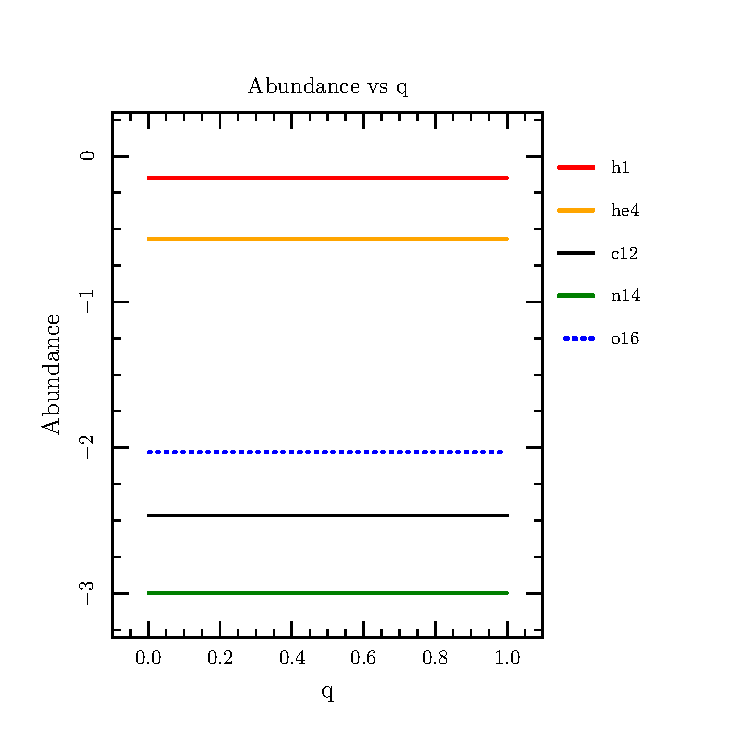
\includegraphics[width = 5in]{/Users/jaredbrooks/brown_dwarf/plots_out/Abundance_vs_q.pdf}
		\caption{Abundance profile}
		\label{fig:1}
	\end{figure}

        \pagebreak

        Here on the H.R. Diagram (figure \ref{fig:2}) we see decreasing luminosity throughout the evolution, but a temporary increase in effective temperature early in its evolution.  The brown dwarf contracts, as shown in the plot to the right (figure \ref{fig:3}).

        \begin{figure}[H]
                \begin{minipage}[b]{0.5\linewidth}
                       \centering
                       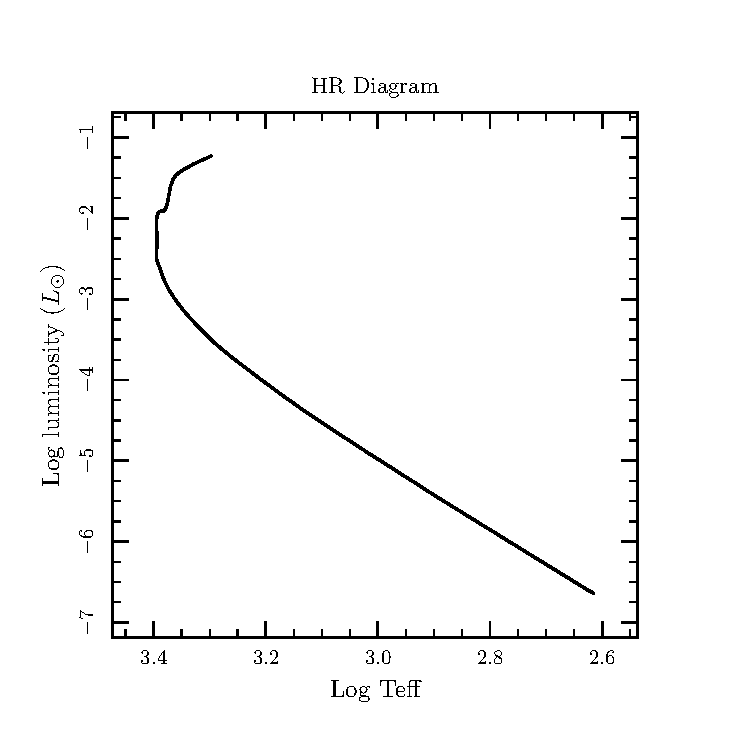
\includegraphics[width = 3.65in]{/Users/jaredbrooks/brown_dwarf/plots_out/HR_Diagram.pdf}
                       \caption{\footnotesize H.R. Diagram where the evolution track goes from top to bottom}
                       \label{fig:2}
                \end{minipage}
                \hspace{0cm}
                \begin{minipage}[b]{0.5\linewidth}
                       \centering
                       \includegraphics[width = 3.65in]{/Users/jaredbrooks/brown_dwarf/plots_out/Log_R_vs_Age.pdf}
                       \caption{\footnotesize Gravitational potential energy is released as the star contracts, leading to slight rise in effective temperature}
                       \label{fig:3}
                \end{minipage}
        \end{figure}

        This next plot to the left (figure \ref{fig:4}) similarly shows effective temperature behavior, but against log[g], and a profile of temperature vs. density at several different ages (figure \ref{fig:5}).

        \begin{figure}[H]
                \begin{minipage}{0.5\linewidth}
                       \centering
                       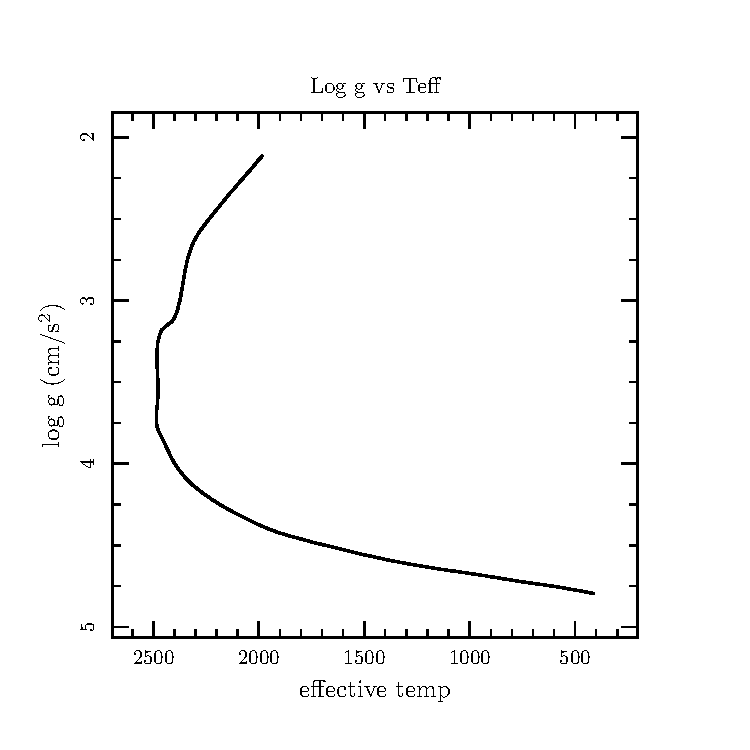
\includegraphics[width = 3.65in]{/Users/jaredbrooks/brown_dwarf/plots_out/log_g_vs_Teff.pdf}
                       \caption{\footnotesize Log g vs. effective T where the evolution track goes from top to bottom}
                       \label{fig:4}
                       \end{minipage}
                \hspace{0cm}
                \begin{minipage}{0.5\linewidth}
                       \centering
                       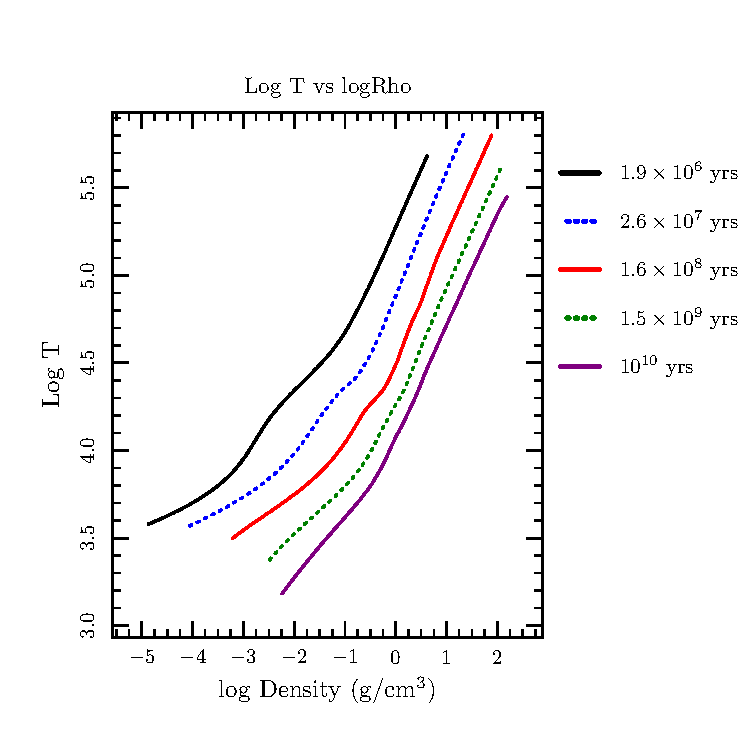
\includegraphics[width = 3.65in]{/Users/jaredbrooks/brown_dwarf/plots_out/Log_T_vs_logRho.pdf}
                       \caption{\footnotesize Temperature vs. density profile at several ages show increase in density and temporary bump in temperature}
                       \label{fig:5}
                \end{minipage}
        \end{figure}

        This next plot (figure \ref{fig:7}) was taken from a convergence study.  The C value is proportional to the spatial and temporal resolution controls, where higher C values correspond to lower resolution, and vice versa.  The error is RMS error taken at 5 ages (1 Myr, 10 Myr, 100Myr, 1 Gyr, 10 Gyr) relative to the lowest C value used, which is C=0.1.

        \begin{figure}[H]
                \centering
                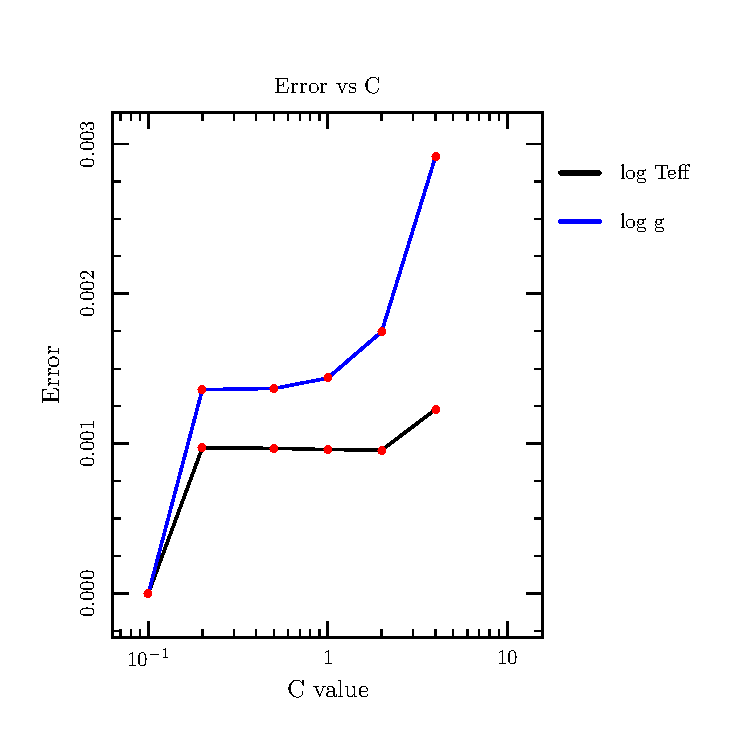
\includegraphics[width = 5in]{/Users/jaredbrooks/brown_dwarf/plots_out/Error_vs_C_0-02.pdf}
                \caption{RMS error vs C, where C is inverse of resolution}
                \label{fig:7}
        \end{figure}

        \pagebreak

        This final plot (figure \ref{fig:6}) shows a few internal \texttt{MESA} variables, such as the size of the time-step, the number of zones, and the number of retries against the model number in order to give some understanding of how hard \texttt{MESA} is working throughout the run and where some areas of problems/interest might be.

        \begin{figure}[H]
                \centering
                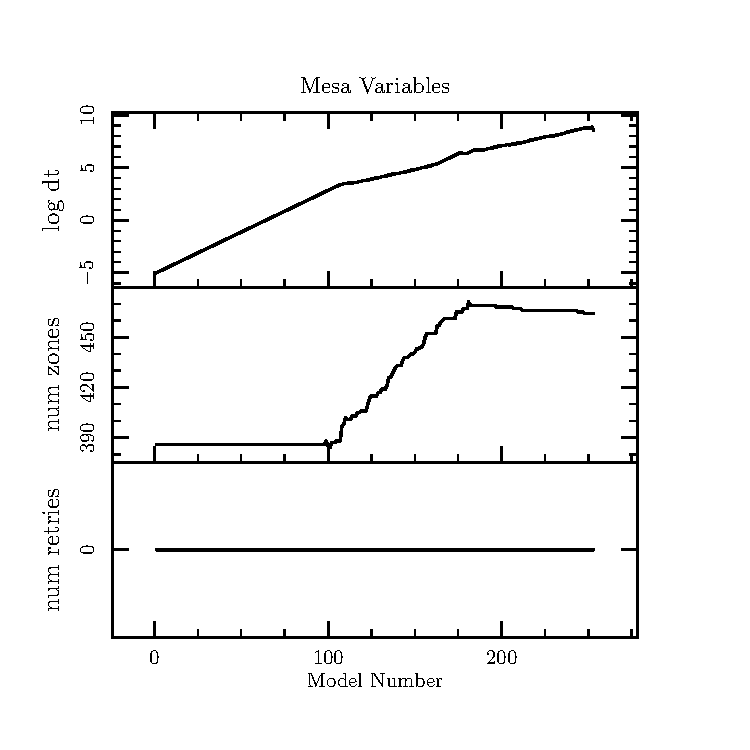
\includegraphics[width = 5in]{/Users/jaredbrooks/brown_dwarf/plots_out/Mesa_Variables.pdf}
                \caption{\texttt{MESA} variables plotted against model number show how hard \texttt{MESA} is working}
                \label{fig:6}
        \end{figure}

\end{document}
